\section*{Лекция 10 (21.04.2022)}

\subsection{Производные высших порядков}

\begin{enumerate}
    \item (Самая простая ситуация)
	\begin{definition}
    \[
        f : \R^m \to \R, \text{ дифференцируема на всем } \R^m \hence \exists \frac{\partial f}{\partial x_j} : \R ^m \to \R 
    \]

    Может оказаться, что $\frac{\partial f}{\partial x_j}$ дифф. $\hence \exists \frac{\partial }{\partial x_k} \left( \frac{\partial f}{\partial x_j} \right)$ --- вторая частная производная

    Далее по индукции. Аналогичные записи:

    \[
        \frac{\partial }{\partial x_k} \left( \frac{\partial f}{\partial x_j} \right) = \frac{\partial ^ 2 f}{\partial x_k \partial x_j}(x) = D^2_{x_k, x_j} f(x)
    \]

    \[
        \frac{\partial ^ pf}{\partial x_{i_p} ... \partial x_{i_1}} \text{ --- производная p-го порядка}
    \]
	\end{definition}

    \begin{theorem}
        $f: \R ^ m \to \R, x \in \R ^m, $ существуют частные проивзодные $\frac{\partial ^ 2f}{\partial x_k \partial x_j}$ и $\frac{\partial ^ 2 f}{\partial x_j \partial x_k}$ в окр. $(\cdot)$ x и оказались непр. в $(\cdot)$ x $\hence \frac{\partial ^ 2f}{\partial x_k \partial x_j} = \frac{\partial ^ 2 f}{\partial x_j \partial x_k}$.
    \end{theorem}

    \begin{remark} (Напоминание)
        $\frac{\partial f}{\partial x_j}(x) = \lim_{t \to 0} \frac{f(x + t e_j) - f(x)}{t}$
    \end{remark}

    \begin{proof}
        Считаем, что только 2 переменных $x_1, x_2$.

        \[
            F(h_1, h_2) = f(x_1 + h_1, x_2 + h_2) - f(x_1 + h_1, x_2) - f(x _ 1, x_2 + h_2) + f(x_1, x_2)
        \]

        
\newpage
\tikzset{every picture/.style={line width=0.75pt}} %set default line width to 0.75pt        

\begin{tikzpicture}[x=0.75pt,y=0.75pt,yscale=-1,xscale=1]
%uncomment if require: \path (0,300); %set diagram left start at 0, and has height of 300

%Shape: Rectangle [id:dp6515847412486357] 
\draw   (100,126) -- (383,126) -- (383,232) -- (100,232) -- cycle ;
%Straight Lines [id:da7289755314944631] 
\draw    (99,181) -- (380,181) ;

% Text Node
\draw (61,240.4) node [anchor=north west][inner sep=0.75pt]    {$+ ( x_{1} ,x_{2})$};
% Text Node
\draw (389,82.4) node [anchor=north west][inner sep=0.75pt]    {$+ ( x_{1} +h_{1} ,x_{2} +h_{2})$};
% Text Node
\draw (385,235.4) node [anchor=north west][inner sep=0.75pt]    {$- ( x_{1} +h_{1} ,x_{2})$};
% Text Node
\draw (58,98.4) node [anchor=north west][inner sep=0.75pt]    {$- ( x_{1} ,x_{2} +h_{2})$};
% Text Node
\draw (397,170.4) node [anchor=north west][inner sep=0.75pt]    {$t\in [ 0,\ 1]$};
% Text Node
\draw (-1,170.4) node [anchor=north west][inner sep=0.75pt]    {$( x_{1} ,\ x_{2} +th_{2})$};


\end{tikzpicture}

\[
    \phi(t) = f(x_1 + h_1, x_2 + th_2) - f(x_1, x_2 + th_2)
\]

\[
    F(h_1, h_2) = \phi(1) - \phi(0) = \phi'(\theta_2)
\]

\[
    \phi'(\theta_2) = \frac{\partial f}{\partial x_2} (x_1 + h_1, x_2 + \theta_2 h_2) \cdot h_2 - \frac{\partial f}{\partial x_2}(x_1, x_2 + \theta_2 h_2) \cdot h_2 \overset{\exists \theta_1}{=} \frac{\partial}{\partial x_1} \left (\frac{\partial f}{\partial x_2}\right ) (x_1 + \theta_1 \cdot h_1, x_2 + \theta_2 h_2) h_2 h_1
\]

\[
     \frac{F(h_1, h_2)}{h_1 h_2} \underset{h \to 0}{\to} \frac{\partial ^ 2 f}{\partial x_1 \partial x_2}(x)
\]

По аналогии можно получить, что 
\[
	\frac{F(h_1, h_2)}{h_1 h_2} \underset{h \to 0}{\to} \frac{\partial ^ 2 f}{\partial x_2 \partial x_1}(x)
\]
    \end{proof}

    \follow\, Если у функции существуют непрерывные проивзодные $n$-ого порядка $\hence  \frac{\partial ^n f}{\partial x_{i_n}... \partial x_{i_1}} (x) = \frac{\partial ^ n f}{\partial x_{\sigma(n)} ... \partial x_{i_{\sigma(1)}} } \forall \sigma \in S_n$

    \item 
	\begin{definition}
	
	$f : X \to Y$, f дифференцируема на X (в окрестности $(\cdot) x$)
    
    $df : X \to L(X, Y)$ может оказаться, что $df$ дифференцируема в $\point$ x.

    $d(df)(x) = L(X; L(X, Y)) \cong L(X, X ; Y)$ --- пространство непрерывных билинейных отображений из $X \times X $ в Y.
    
    $d(df)(x) = d^2 f(x)$ --- второй диференциал $f$ в $\point$ x.

    Но по хорошему это: $d^2 f(x) (h_1, h_2)$

    По индукции определяется $n$-ый дифференциал.

    $d ^ n f(x) \in L(\underbrace{X, X, ... , X}_{n}; Y)$
	\end{definition}


	\begin{theorem}[Связь с производными по векторам]

    \[
        df(x) h = \frac{\partial f}{\partial h}(x) = \lim_{t \to 0} \frac{f(x + th) - f(x)}{t} \Longleftrightarrow  f(x + th) - f(x) = df(x) th + o(t)
    \]

    \[
        d ^ 2 f(x) (h_1, h_2) = (d(df) (x) h_1) h_2 = \left (\frac{\partial}{\partial h_1} (df)(x)\right) h_2 = \left(\lim_{t \to 0} \frac{df(x + th_1) - df(x)}{t} \right) h_2 \ceq
    \]

    \[
        \begin{cases}
            d(df)(x) : X \to L(X, Y)\\
            d(df)(x)h_1 \in L(X, Y)
        \end{cases}
    \] 

    \begin{remark}
        $A_n \to A_0$ в $L(X, Y) \hence \forall h, A_n h \to A_0 h $, т.к. $\norm{A_n h - A_0 h} \leqslant \norm{A_n - A_0} \cdot \norm{h}$
    \end{remark}

    \[
        \ceq \lim_{t \to 0} \frac{df(x + th_1) h_2 - df(x)h_2}{t} = \lim_{t \to 0} \frac{\frac{\partial f(x + th_1)}{\partial h_2} - \frac{\partial f(x)}{\partial h_2}}{t} = \frac{\partial}{\partial h_1} \left(\frac{\partial f}{\partial h_2} \right) (x)
    \]

    \[
        d ^ n f(x) (h_1, ..., h_n) = \frac{\partial }{\partial h_1} \left( \frac{\partial}{\partial h_2} \left(... \left(\frac{\partial f}{\partial h_n} \right)\right) \right)(x)
    \]

	\end{theorem}

    \begin{theorem}[симметричность формы $n$-ого дифференциала]
        
        Если $\exists d^n f(x)$ --- определенный в окрестности точки x и непрерывно зависящий от x, то $d^n f(x)(h_1, ..., h_n) = d^n f(x) (h_{\sigma(1)}, ..., h_{\sigma(n)}) \forall \sigma \in S_n$ 
    \end{theorem}

    \begin{proof}
        $n = 2$ Проверим, что \[ 
            \frac{\partial}{\partial h_1} \frac{\partial}{\partial h_2} f(x) = \frac{\partial }{\partial h_2} \frac{\partial}{\partial h_1} f(x)
        \]



        \tikzset{every picture/.style={line width=0.75pt}} %set default line width to 0.75pt        

        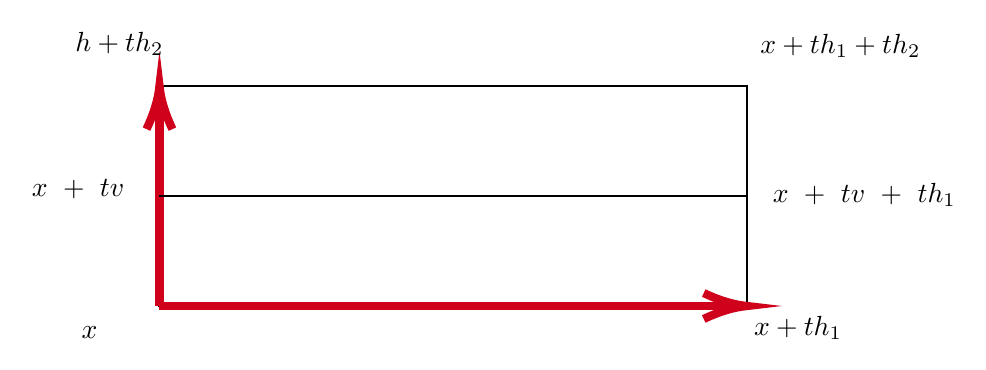
\begin{tikzpicture}[x=0.75pt,y=0.75pt,yscale=-1,xscale=1]
        %uncomment if require: \path (0,300); %set diagram left start at 0, and has height of 300
        
        %Shape: Rectangle [id:dp6515847412486357] 
        \draw   (100,126) -- (383,126) -- (383,232) -- (100,232) -- cycle ;
        %Straight Lines [id:da34567687403467606] 
        \draw [color={rgb, 255:red, 208; green, 2; blue, 27 }  ,draw opacity=1 ][line width=3]    (100,232) -- (100,131) ;
        \draw [shift={(100,126)}, rotate = 90] [color={rgb, 255:red, 208; green, 2; blue, 27 }  ,draw opacity=1 ][line width=3]    (20.77,-6.25) .. controls (13.2,-2.65) and (6.28,-0.57) .. (0,0) .. controls (6.28,0.57) and (13.2,2.66) .. (20.77,6.25)   ;
        %Straight Lines [id:da9577906398624345] 
        \draw [color={rgb, 255:red, 208; green, 2; blue, 27 }  ,draw opacity=1 ][line width=3]    (100,232) -- (378,232) ;
        \draw [shift={(383,232)}, rotate = 180] [color={rgb, 255:red, 208; green, 2; blue, 27 }  ,draw opacity=1 ][line width=3]    (20.77,-6.25) .. controls (13.2,-2.65) and (6.28,-0.57) .. (0,0) .. controls (6.28,0.57) and (13.2,2.66) .. (20.77,6.25)   ;
        %Straight Lines [id:da9490137633848582] 
        \draw    (100,179) -- (383,179) ;
        
        % Text Node
        \draw (61,240.4) node [anchor=north west][inner sep=0.75pt]    {$x$};
        % Text Node
        \draw (388,99.4) node [anchor=north west][inner sep=0.75pt]    {$x+th_1+th_2$};
        % Text Node
        \draw (385,235.4) node [anchor=north west][inner sep=0.75pt]    {$x+th_1$};
        % Text Node
        \draw (58,98.4) node [anchor=north west][inner sep=0.75pt]    {$h+th_2$};
        % Text Node
        \draw (37,169.4) node [anchor=north west][inner sep=0.75pt]    {$x\ +\ tv$};
        % Text Node
        \draw (394,171.4) node [anchor=north west][inner sep=0.75pt]    {$x\ +\ tv\ +\ th_{1}$};
        
        
        \end{tikzpicture}


\quad


\[
	v \,||\, h_2 \text{ и } \norm{v} \leqslant \norm{h_2}     
\]

\[
    F(h_1, h_2; t) = f(x + t h_1 + t h_2) - f(x + th_1) - f(x + th_2) + f(x) 
\]

\[
    \phi(v) = f(x + tv + th_1) - f(x + tv)
\]

\[
    F(h_1, h_2, t) = \phi(h_2) - \phi(0)
\]

\[
    \norm{F(h_1, h_2, t) - t ^ 2 d ^ 2 f(x) (h_1, h_2)} \overset{?}{=} o(t^2) 
\]

\[
	\norm{F(h_1, h_2, t) - t ^ 2 d ^ 2 f(x) (h_1, h_2)} = \norm{\phi(h_2) - \phi(0) - t^2 d^2 f(x) (h1) h_2} \leqslant
\]

\[ \text{(теорема о конечном приращении)} \leqslant \sup_{\theta_2 \in (0, 1) } \norm{\underbrace{d\phi(\theta_2  h_2)}_{d\phi(\theta_2h_2)=(df(x+\theta_2h_2t+th_1)-df(x+\theta_2h_2t))t} - t^2 d^2 f(x) (h_1)} \norm{h_2} \ceq
\]


\[
    \ceq \abs{t} \norm{h_2} \sup_{\theta_2} \norm{\underbrace{df(x + \theta_2 h_2 t + t h_1) - df(x + \theta_2 h_2 t)}_{=d (df) (x + \theta_2 h_2 t) t h_1 + o(t h_1)} - t d(df)(x)h_1} =
\]

\[
	=\left[\text{по непрерывности } d(df)(x) \right] = \abs{t}^2 \norm{h_2} \sup_{\theta_2} \norm{o(1) \cdot h1} = o(t^2), t \to 0	
\]
 Альтернативный вариант, еще раз применяем теорему о конечном приращении:
\[
    \leqslant \abs{t} \norm{h_2} \sup_{\theta_2}  \sup_{\theta_1} \norm{
        d(df)(x + \theta_2 h_2 t + \theta_1 t h_1) - d(df)(x)
    } \cdot \norm{t h_1} = o(t^2), t \to 0
\]


\[
    \Rightarrow \frac{F(h_1, h_2, t)}{t ^ 2} \underset{t \to 0} {\to} d^2 f(x) (h_1, h_2)
\]
    \end{proof}
\end{enumerate}

\underline{Частный случай} $f : \R^m \to \R$

\[
    h_k = h^{(1)}_k e_1 + ... + h^{(m)}_k e_m
\]

\[
    d^n f(x) (h_1, ..., h_n) = 
    d ^ n f(x) \left(\sum_{j = 1}^m h_1^{(j)}e_j, ..., \sum_{j = 1}^m h_n^{(j)} e_j \right) = 
    \sum_{1 \leqslant j_1 \dots j_n \leqslant m} \underbrace{d^n f(x) (e_{j_1}, ... ,e_{j_n})}_{\frac{\partial ^ n f}{\partial x_{j_1} ... \partial x_{j_n}}(x) } h_1^{(j_1)} \cdot ... \cdot h_n ^ {(j_n)}
\]

$
    n = 2, m = 2
$

\[
    d ^ 2 f(x, y) \begin{pmatrix}
        h_1^{(1)}&h_2^{(1)}\\
        h_1^{(2)}&h_2^{(2)}
    \end{pmatrix} = 
    \frac{\partial ^ 2 f}{\partial x ^ 2}(x, y) h_1^{(1)} h_2^{(1)} +
    \frac{\partial ^ 2 f}{\partial y ^ 2}(x, y)
    h_1^{(2)} h_2^{(2)} +
    \frac{\partial ^ 2 f}{\partial x \partial y} (x, y) (h_1 ^ {(1)} h_2 ^ {(2)} + h_1 ^ {(2)} h_2 ^ {(1)})
\]

\[
    d^n  f(x) = \sum_{1 \leqslant j_1 ... j_n \leqslant m} \frac{\partial ^ n f(x)}{\partial x_{j_1} ... \partial x_{j_n}} d x_{j_1} ... dx_{j_n}
\]

\[
    d ^ 2 f(x, y) = \frac{\partial ^ 2 f}{\partial x ^ 2} dx dx + \frac{\partial^2 f}{\partial x \partial y }(dx dy + dy dx) + \frac{\partial ^ 2 }{\partial y ^ 2}  dy dy =
    \left (\frac{\partial}{\partial x} dx + \frac{\partial }{\partial y} dy \right) ^ 2 f(x, y)
\]

\[
    d^n f(x) = \left( \frac{\partial}{\partial x_1} dx_1 + ... + \frac{\partial}{\partial x_m} dx_m  \right) ^ n f(x)
\]

\quad

\textbf{Важный случай:}  $h_1 = h_2 = ... = h_n$

\[
    d ^ n f(x) (h, h, ..., h) = d ^ n f(x) h ^ n
\]

\[
    d ^ n f(x) (h, h, ..., h) = \sum_{\alpha_1, ..., \alpha_m, \alpha_1 + ... + \alpha_m = n, \alpha_j \in \Z_{\geqslant 0}} \frac{n !}{\alpha_1 ! ... \alpha_m !}
     \frac{\partial ^ n}{(\partial x_1) ^ {\al_1} ... (\partial x_m) ^ {\al_m}} (x) (h ^ {(1)}) ^ {\al_1} \cdot ... \cdot (h ^ {(m)}) ^ {\al_m}
\]
\[     
	 = \sum_{\abs{\al} = n} \frac{n !}{\al !} \frac{\partial ^ n f(x)}{\partial x ^ \al} h ^ \al
\]

$\al$ --- мультииндекс

$h^\al = h^{(1)^{\al_1}} ... h^{(m)^{\al_m}}$

$\al ! = \al_1 ! ... \al_m !$

$\abs{\al} = n$ --- высота (поярдок) мультииндекса

\[
    d ^ n f(x) = \sum_{\alpha : \abs{\al} = n}
    \frac{n !}{\al !} \frac{\partial ^ n f(x)}{\partial x ^ \al} (dx) ^ \al
\]

Второй дифференциал

\[
    d ^ 2 f(x) (h, h) = \langle H(x) h, h \rangle
\]

$H(x)$ --- матрица Гесса 

$H(x) = (\frac{\partial ^ 2 f}{\partial x_i \partial x_j}(x))$

\underline{Выпуклость}

$\langle H(x) h, h \rangle \geqslant 0 \Longleftrightarrow \frac{\partial ^2 f}{\partial h^2}(x) \geqslant 0$

\subsection{Многомерная формула Тейлора}

\begin{theorem}[Формула Тейлора]
    $f : \R ^ m \to \R$, $f$ ~--- $n + 1$ раз непрерывно дифференцируема на $[x, x + h]$.

	\[
		f(x + h) = f(x) + \sum_{k = 1} ^ n \frac{d ^ k f(x) h ^ k}{k !} + \frac{d ^ {n + 1} f(x + \theta h) h ^ {n + 1}}{(n + 1)!}, \exists \theta \in (0, 1)
	\]
\end{theorem}

\begin{proof}
    $\phi(t) = f(x + th)$, $\phi$ $n + 1$ раз дифференцируема на $[0, 1] \Rightarrow$

	\[
		\underbrace{\phi(1)}_{f(x + h)} = \underbrace{\phi(0)}_{f(x)} + \sum_{k = 1} ^ n \frac{\phi^{(k)} (0)}{k !} + \frac{\phi^{(n + 1)}(\theta)}{(n + 1)!}
	\]


    \[
        \phi^{(k)}(t) = d^{(k)} f(x + th) h ^ k
    \]

    Пояснение на следующей лекции.
\end{proof}
